\chapter{Advice for applying  machine learning}
\section{Evaluating a model}
\subsection*{Training and testing set}
Split the data into two sets: a training set and a testing set. The training set is used to train the model, 
and the testing set is used to evaluate the model. 
The testing set should be large enough to give a good estimate of the model's performance.
 A common split is 80\% training and 20\% testing.\\
\includegraphics*[width=\textwidth]{images/10.1}
\par
\noindent
{\large \textbf{Compute the error}:}\\
\textbf{For regression:}
\begin{itemize}
    \item $m_{train} = m_1$, $m_{test} = m_2$
    \item Fit parameters by minimizing the error cost function on the training set:
    \[ J(\mathbf{w}, b) = \frac{1}{2m_1} \sum_{i=1}^{m_1} (f_{\mathbf{w}, b}(x^{(i)}) - y^{(i)})^2 + 
    \frac{\lambda}{2m_1}\sum_{i=1}^{n}w_j^2\]
    note: the second term is the regularization term.
    \item Compute the error on the test set:
    \[ J_{test}(\mathbf{w}, b) = \frac{1}{2m_2} \sum_{i=1}^{m_2} \left(f_{\mathbf{w}, b}(x^{(i)}) - y^{(i)}\right)^2 \]
    note: the regularization term is not included in the test error.
    \item compute the training error:
    \[ J_{train}(\mathbf{w}, b) = \frac{1}{2m_1} \sum_{i=1}^{m_1} \left(f_{\mathbf{w}, b}(x^{(i)}) - y^{(i)}\right)^2 \]
\end{itemize}
\par
\textbf{For classification:}
\begin{itemize}
    \item $m_{train} = m_1$, $m_{test} = m_2$
    \item Fit parameters by minimizing the error cost function on the training set:
    \[ J(\mathbf{w}, b) = -\frac{1}{m_1} \sum_{i=1}^{m_1} \left[y^{(i)}\log\left(f_{\mathbf{w}, b}(x^{(i)})\right) + (1-y^{(i)})\log\left(1-f_{\mathbf{w}, b}(x^{(i)})\right)\right]
    + \frac{\lambda}{2m_1}\sum_{i=1}^{n}w_j^2\]
    note: the second term is the regularization term.
    \item Compute the error on the test set:
    \[ J_{test}(\mathbf{w}, b) = -\frac{1}{m_2} \sum_{i=1}^{m_2} \left[y^{(i)}\log\left(f_{\mathbf{w}, b}(x^{(i)})\right) + (1-y^{(i)})\log\left(1-f_{\mathbf{w}, b}(x^{(i)})\right)\right] \]
    \item compute the training error:
    \[ J_{train}(\mathbf{w}, b) = -\frac{1}{m_1} \sum_{i=1}^{m_1} \left[y^{(i)}\log\left(f_{\mathbf{w}, b}(x^{(i)})\right) + (1-y^{(i)})\log\left(1-f_{\mathbf{w}, b}(x^{(i)})\right)\right] \]
\end{itemize}
\par
\begin{notebox}
    \hspace{2em}There is another way to compute the error for classification, which is more common in practice. 
    The testing/training error is the fraction of the test/train set that has been misclassified:
    \begin{itemize}
        \item Compute the error on the test set:
        \[ J_{test}(\mathbf{w}, b) = \frac{1}{m_2} \sum_{i=1}^{m_2} \mathbf{1}\left\{y^{(i)} \neq \text{prediction}\right\} \]
        \item compute the training error:
        \[ J_{train}(\mathbf{w}, b) = \frac{1}{m_1} \sum_{i=1}^{m_1} \mathbf{1}\left\{y^{(i)} \neq \text{prediction}\right\} \]
        \item[] where $\mathbf{1}\left\{y^{(i)} \neq \text{prediction}\right\}$ is an indicator function that is 1 if the prediction is wrong and 0 if the prediction is correct.
        \item[] This is called the 0/1 misclassification error.
    \end{itemize}
\end{notebox}
\par
Usually, the training error is lower than the test error, because the model is trained to minimize the training error.
\subsection*{model selection}
\begin{minipage}{0.51\textwidth}
\begin{enumerate}
    \item $f_{\mathbf{w}, b} = w_1x + b$
    \item $f_{\mathbf{w}, b} = w_1x + w_2x^2 + b$
    \item $f_{\mathbf{w}, b} = w_1x + w_2x^2 + w_3x^3 + b$
    \item[] \hspace{3em}$\vdots$
    \item[10.] $f_{\mathbf{w}, b} = w_1x + w_2x^2 + \cdots + w_{10}x^{10} + b$
\end{enumerate}
\end{minipage}
\vrule{}
\begin{minipage}{0.2\textwidth}
\begin{enumerate}
    \item $w^{\langle1\rangle}, b^{\langle1\rangle}$
    \item $w^{\langle2\rangle}, b^{\langle2\rangle}$
    \item $w^{\langle3\rangle}, b^{\langle3\rangle}$
    \item[] \hspace{1em}$\vdots$
    \item[10.] $w^{\langle10\rangle}, b^{\langle10\rangle}$
\end{enumerate}
\end{minipage}
\vrule{}
\begin{minipage}{0.25\textwidth}
\begin{enumerate}
    \item $J_{\text{test}}(w^{\langle1\rangle}, b^{\langle1\rangle})$
    \item $J_{\text{test}}(w^{\langle2\rangle}, b^{\langle2\rangle})$
    \item $J_{\text{test}}(w^{\langle3\rangle}, b^{\langle3\rangle})$
    \item[] \hspace{1em}$\vdots$
    \item[10.] $J_{\text{test}}(w^{\langle10\rangle}, b^{\langle10\rangle})$
\end{enumerate}
\end{minipage}
\par
Assume that the $J_{\text{test}}(w^{\langle5\rangle}, b^{\langle5\rangle})$ is the smallest, then we choose the model
with $d = 5$.\par
However, this method has flaws. If we want to get the generalization error, the problem is that 
$J_{\text{test}}(w^{\langle5\rangle}, b^{\langle5\rangle})$ is likely to be an overly optimistic estimate of 
generalization error(how well the model will perform on new data), which is to say $J_{\text{test}}(w^{\langle5\rangle}, b^{\langle5\rangle})< \text{generalization error}$.
\par
This is because the extra parameter $d$ was chosen using the test set. Just like choosing $w, b$ from the training set,
$w, b$ are overly optimistic estimate of the generalization error.
\newpage
\subsection*{Cross-validation}
Split the data into three sets: a training set, a cross-validation set, and a testing set.\par
\vspace{2em}
\includegraphics*[width=\textwidth]{images/10.3}
\textbf{Compute the error:}\par
The same method as before, but now we will compute the cross-validation error:
\[J_cv(\mathbf{w}, b) = \frac{1}{2m_{cv}} \sum_{i=1}^{m_{cv}} \left(f_{\mathbf{w}, b}(x_{cv}^{(i)}) - y_{cv}^{(i)}\right)^2\]
\includegraphics*[width=\textwidth]{images/10.4}
\newpage
\noindent
{\large \textbf{Model selection:}}\par
Most parts are the same as before, but now we will choose the model with the smallest cross-validation error.\\
\includegraphics*[width=\textwidth]{images/10.5}
\par
It also can be applied to neural networks.\\
\includegraphics*[width=\textwidth]{images/10.6}
\newpage
\section{Bias and variance}
\begin{dfnbox}{Bias}{b}
    \textbf{Bias} refers to the error that is introduced by approximating a real-life problem by a much simpler model, which may be extremely complex.
    Often, the model is too simple to capture the underlying structure of the data. This situation is called \textbf{underfitting}.
    And the indicator of bias is the training error. If the training error is high, then the model may have high bias.
\end{dfnbox}
\begin{dfnbox}{Variance}{v}
    \textbf{Variance} refers to the error that is introduced by approximating a real-life problem by a much more complex model.
    Often, the model is too complex to capture the underlying structure of the data. This situation is called \textbf{overfitting}.
    And the indicator of variance is the gap between the training error and the cross-validation error. If the gap is large, then the model may have high variance.
\end{dfnbox}
\includegraphics*[width=\textwidth]{images/10.7}
\begin{itemize}
    \item High Bias (underfit):
    \item[] $J_{\text{train}}$ will be high and $J_{\text{cv}} \approx J_{\text{train}}$.
    \item High Variance (overfit):
    \item[] $J_{\text{cv}} \gg J_{\text{train}}$ and $J_{\text{train}}$ may be low.
    \item High Bias and High Variance:
    \item[] $J_{\text{cv}} \gg J_{\text{train}}$ and $J_{\text{train}}$ is high.
\end{itemize}
\includegraphics*[width=\textwidth]{images/10.8}
\subsection*{Regularization}
We can use the error $J_{\text{train}}$ and $J_{\text{cv}}$ to choose the regularization 
parameter $\lambda$.\\
\includegraphics*[width=\textwidth]{images/10.9}
\includegraphics*[width=\textwidth]{images/10.10}
\par
The two graphs are important.
Notice the difference between the two, the first one's variable is $\lambda$, 
and the second one's variable is ``degree of polynomial''.\\
\includegraphics*[width=\textwidth]{images/10.11}
\section{Baseline level of performance}
Establishing a baseline level of performance is important.
 It can be used to compare the performance of your model.\par
There are some ways to establish a baseline level of performance:
\begin{itemize}
    \item Human-level performance: the error rate that a human can achieve.
    \item Competing algorithms performance
    \item Guess based on experience
\end{itemize}
\par
The baseline performance can be used to diagnose bias and variance.
\begin{itemize}
    \item If the gap between the training error and the baseline performance is large,
    then the model may have high bias.
    \item If the gap beween the cross validation error and the training error is large,
    then the model may have high variance.
\end{itemize}
\includegraphics*[width=\textwidth]{images/10.12}
\section{Learning curves}
Usually, as the number of training examples increases, 
the cross-validation error will decrease while the training error will increase.
\\
\includegraphics*[width=\textwidth]{images/10.13}
\subsection*{High bias}
As the training data increases, $J_cv$ and $J_train$ will become flat, but still have a gap beween the
baseline performance.\\
\includegraphics*[width=\textwidth]{images/10.14}
\par
Because of that, getting more training data will not help much.
\subsection*{High variance}
As the traing data increases, $J_cv$ and $J_train$ will become closer to the baseline performance.\\
\includegraphics*[width=\textwidth]{images/10.15}
\par
High variance can be solved by lifting the size of training set, 
but this process may take a large amount of data.
\subsection*{Debug a learning algorithm}
\begin{minipage}{0.6\textwidth}
    \begin{itemize}
        \item Get more training examples
        \item Try smaller sets of features
        \item Try getting additional features
        \item Try adding polynomial features($x_1^2, x_2^2, x_1x_2, \cdots$)
        \item Try decreasing $\lambda$
        \item Try increasing $\lambda$
    \end{itemize}
\end{minipage}
\begin{minipage}{0.4\textwidth}
    \begin{itemize}
        \item[] fix high variance
        \item[] fix high variance
        \item[] fix high bias
        \item[] fix high bias
        \item[] fix high bias
        \item[] fix high variance
    \end{itemize}
\end{minipage}
\includegraphics*[width=\textwidth]{images/10.16}
\subsection*{Neural networks}
A large neural network often has low bias, and it will usually do well or better than a smaller neural network
as long as regularization is used to control overfitting.
\\
\includegraphics*[width=\textwidth]{images/10.17}
\par
\begin{minted}{python}
    layer_1 = Dense(units=25, activation='relu', kernel_regularizer=L2(0.01))
    layer_2 = Dense(units=15, activation='relu', kernel_regularizer=L2(0.01))
    layer_3 = Dense(units=1, activation='sigmoid', kernel_regularizer=L2(0.01))
    model = Sequential([layer_1, layer_2, layer_3])
\end{minted}
\par
The code above is an example of how to add regularization to a neural network. 
The \texttt{kernel\_regularizer} parameter is used to add regularization to the weights of the layer.

\section{Machine learning develop process}
\subsection*{Iterative loop of machine learning}
\includegraphics*[width=\textwidth]{images/10.18}
\subsection*{Error analysis}
\begin{itemize}
    \item Get a lot of ideas
    \item Use error analysis to prioritize ideas
    \item Error analysis means manually examining the examples in the cross-validation set that the algorithm made errors on.
    \item Error analysis can give you insights into what to do next.
\end{itemize}
\subsection*{Adding data}
\noindent
\textbf{Data augmentation:}\\
\includegraphics*[width=\textwidth]{images/10.19}
\includegraphics*[width=\textwidth]{images/10.20}
\includegraphics*[width=\textwidth]{images/10.21}
\includegraphics*[width=\textwidth]{images/10.22}
\includegraphics*[width=\textwidth]{images/10.23}
\subsection*{Transfer learning}
Transfer learning has 2 steps: \textbf{supervised pretraining} and \textbf{fine-tuning}.
We can use a pre-trained model and fine-tune it to our problem. To do it, we can only change the output layer of the model.\\
\includegraphics*[width=\textwidth]{images/10.24}
\par
The reason for that is when input are of the same type, the first few layers of the neural network will learn features that are useful for the new task.
Taking the CV model as an example, the first few layers will learn features that are general to all images such as edges, shapes, etc.
\\
\includegraphics*[width=\textwidth]{images/10.25}
\includegraphics*[width=\textwidth]{images/10.26}
\subsection*{Full cycle of machine learning project}
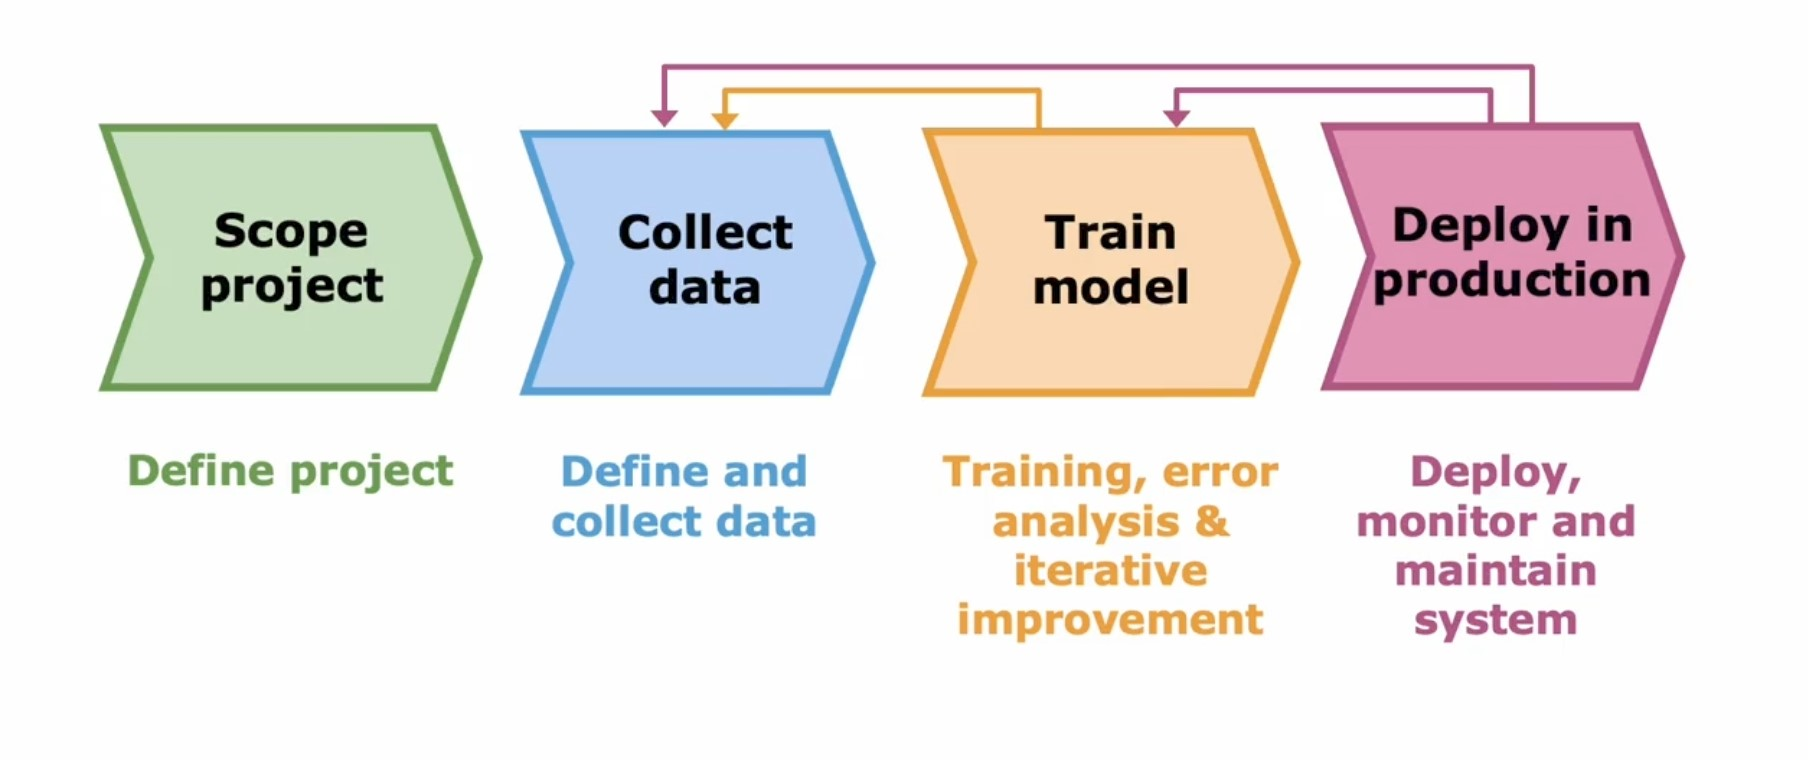
\includegraphics[width=\textwidth]{images/10.27}
\section{Skewed datasets}
\subsection*{Error metrics for skewed datasets}
Skewed datasets are datasets where the classes are not represented equally. For example, in a cancer dataset,
the number of patients with cancer is much smaller than the number of patients without cancer.
\par
In skewed datasets, accuracy is not a good metric to evaluate the model.
For instance, if we have a dataset with 99\% of the examples being negative and 1\% being positive,
a model that predicts all examples as negative will have an accuracy of 99\%. While this model has a high accuracy,
it is not useful because it does not predict any positive examples.
\par
Therefore, we need to use other metrics to evaluate the model. We can divide the predictions into four categories:
\begin{itemize}
    \item True positive (TP): the model correctly predicts the positive class.
    \item False positive (FP): the model incorrectly predicts the positive class.
    \item True negative (TN): the model correctly predicts the negative class.
    \item False negative (FN): the model incorrectly predicts the negative class.
\end{itemize}
\par
\begin{center}
    \includegraphics*[width=0.5\textwidth]{images/10.28}
\end{center}
\par
There are 2 metrics that are commonly used to evaluate models on skewed datasets:
\begin{itemize}
    \item Precision: the fraction of positive predictions that are correct.
    \[ \text{Precision} = \frac{\text{True positive}}{\text{total predicted positive}} = \frac{\text{True pos}}{\text{True pos} + \text{False pos}} \]
    \item Recall: the fraction of the positive examples that the model correctly predicts.
    \[ \text{Recall} = \frac{\text{True positive}}{\text{total actual positive}} = \frac{\text{True pos}}{\text{True pos} + \text{False pos}} \]
\end{itemize}
\par
In this case, the ``always negative'' model has a precision of 0 and a recall of 0.(because the numerator of
precision and recall is 0, note: the denominator of precision is also 0, but the precision and recall are defined as 0 in this case)
\par
\subsection*{Trade off between precision and recall}
There is a trade-off between precision and recall. 
We will set a threshold for predicting the positive class. If the probability of the positive class is greater than the threshold,
we will predict the positive class, negative otherwise. 
If we increase the threshold for predicting the positive class,
the precision will increase, but the recall will decrease.\\
\includegraphics*[width=\textwidth]{images/10.29}
\par
\subsection*{F1 score}
The F1 score is the harmonic mean of precision and recall.
\begin{thmbox}{F1 score}{f1}
\begin{align}
    & P := \text{Precision} \qquad R := \text{Recall} \nonumber \\ 
    &\mathrm{F_1\ score} = \frac{2}{\frac{1}{P} + \frac{1}{R}}= 2 \cdot \frac{P \cdot R}{P + R}
\end{align}
\end{thmbox}
\par
\includegraphics*[width=\textwidth]{images/10.30}